\documentclass[10.5pt]{article}
\usepackage{amsmath, amsfonts, amssymb,amsthm}
\usepackage[includeheadfoot]{geometry} % For page dimensions
\usepackage{fancyhdr}
\usepackage{enumerate} % For custom lists
\usepackage{tikz-cd}
\usepackage{graphicx}

\fancyhf{}
\lhead{MAT1300 hw2}
\rhead{Tighe McAsey - 1008309420}
\pagestyle{fancy}

% Page dimensions
\geometry{a4paper, margin=1in}

\theoremstyle{definition}
\newtheorem{pb}{}

% Commands:

\newcommand{\set}[1]{\{#1\}}
\newcommand{\gen}[1]{\langle#1\rangle}
\newcommand{\abs}[1]{\lvert#1\rvert}
\newcommand{\norm}[1]{\lvert\lvert#1\rvert\rvert}
\newcommand{\tand}{\text{ and }}
\newcommand{\tor}{\text{ or }}
\newcommand{\pd}{\frac{\partial}{\partial x_j}}

\begin{document}
    \begin{pb}
        \textbf{(a)}
        \begin{figure}[h]
            \begin{center}
                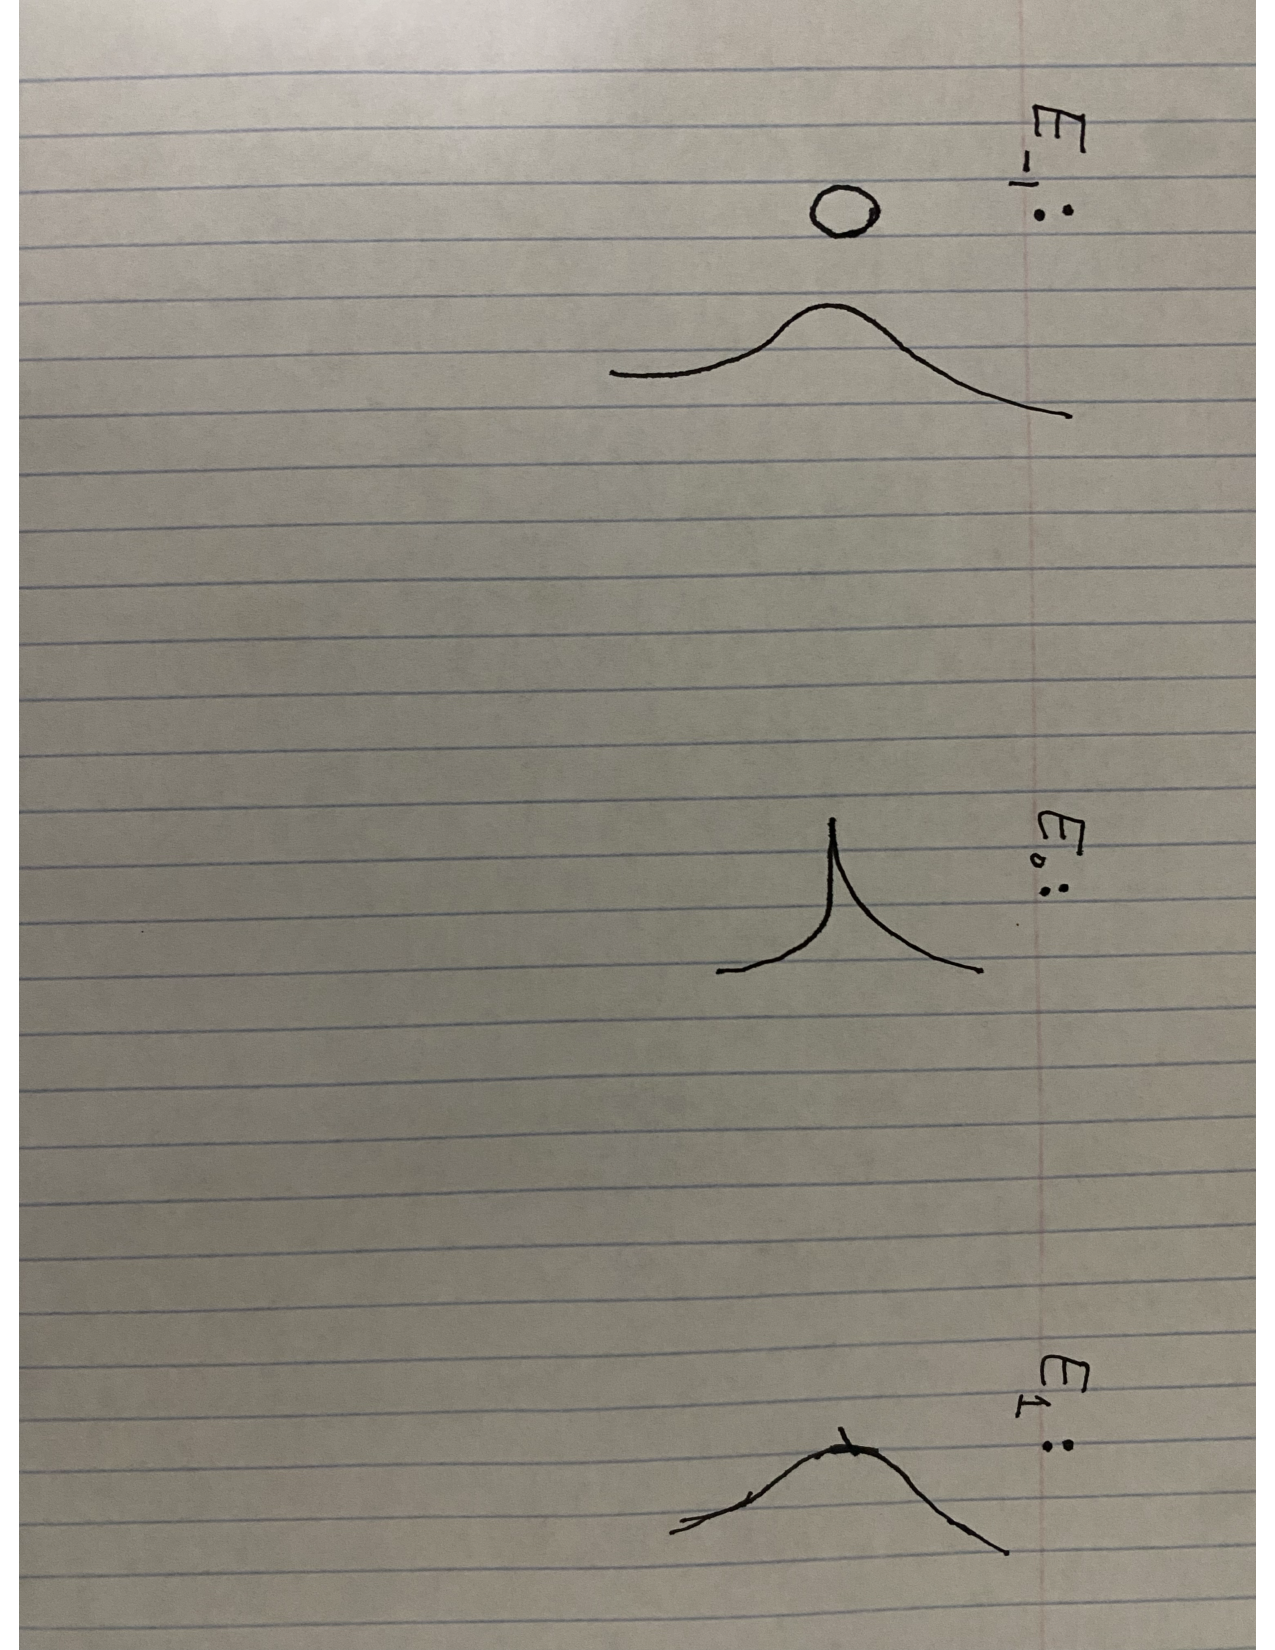
\includegraphics[angle = 90, width = 0.9\linewidth]{EllipticCurveSketch.pdf}
            \end{center}
        \end{figure}

        \textbf{(b)} The set \(\set{y^2 = x^3 + ax}\) is exactly the zero set of \(y^2 - x^3 - ax\), so if \(a \neq 0\) we use the submersion theorem for 
        \begin{align*}
            f : \mathbb{R}^2 &\to \mathbb{R} \\
            (x,y) &\mapsto y^2 - x^3 - ax
        \end{align*}
        Then \(D_{(x,y)}f = \begin{pmatrix} 2y & 3x^2 - a \end{pmatrix}\), this is surjective so long as it is not equal to \(\begin{pmatrix} 0&0 \end{pmatrix}\), but this wont happen since any point where \(y = 0\) on \(E_a\) has \(x = 0\), so surjectivity for all \((x,y)\) follows from \(a \neq 0\). It follows that \(E_a = f^{-1}(0)\) is a submanifold.

        \(E_0\) is not a submanifold, we first show that if it were a submanifold it would have dimension \(1\), note its obvious the dimension can't be zero since \(E_0\) is not a point. Suppose \(E_0\) were to have dimension \(2\), then if \((U,V,\phi)\) were a chart for \(E_0\), containing \((1,1)\) we would have \(\phi: E_0\cap V \overset{\cong}{\to} U\), so that \(\phi: E_0 \cap V \setminus \set{1,1} \to U \setminus \set{\phi(1,1)}\) is also a homeomorphism onto its image, with inverse \(\phi^{-1}\vert_{U \setminus \set{\phi(0,0)}}\), but this is not possible since the former is not connected, and any open subset of \(\mathbb{R}^2\) is still connected after removing a point, so that \(U \setminus \set{\phi(1,1)}\) is not connected.
        
        Now we assume for contradiction that \(E_0\) is a one dimensional submanifold of \(\mathbb{R}^2\), we apply the theorem that a closed set is a submanifold if and only if it is the image of a proper embedding, so we get a proper embedding \(f: E_0 \to \mathbb{R}^2\) with   \(f(\mathbb{R}) = \set{y^2 = x^3}\), and assuming for convenience that \(f(0) = (0,0)\). To see that \(E_0\) cannot be an embedded submanifold, I will show that \(T_0E_0 = 0\), which contradicts \(E_0\) having dimension one. Consider a path \(\gamma:(-\epsilon,\epsilon) \to \mathbb{R}\), then \(f\circ\gamma:(-\epsilon,\epsilon) \to \set{y^2 = x^3} \subset \mathbb{R}^2\), \(t \mapsto (\gamma_1(t),\gamma_2(t))\). By the equation for \(E_0\), we know that \(\gamma_1(t) = \gamma_2(t)^{2/3}\), and hence
        \begin{align*}
            \gamma_1'(0) = \lim_{t\to 0} \gamma_1'(t) = \lim_{t\to 0}\frac23 \gamma_2^{-\frac13}(t)\gamma_2'(t)
        \end{align*}
        Since \(\gamma_2(0) = 0\), we get that the right hand side diverges unless \(\gamma_2'(0) = 0\). Moreover by the equation of \(E_0\), we have \(\gamma_1(t) \geq 0\), and hence
        \begin{align*}
            0 \geq \lim_{t\uparrow 0}\frac{\gamma_1(t)}{t} = \gamma_1'(t) = \lim_{t\downarrow 0}\frac{\gamma_1(t)}{t} \geq 0
        \end{align*}
        so that \(\gamma_1'(t) = 0\), but since \(f\) is an embedding its a diffeomorphism onto its image, so in particular \(([\gamma] \mapsto [f\circ \gamma])\) should be an injection on tangent spaces, but by the chain rule the derivative being zero for an arbitrary path implies that the corresponding derivation is zero, and hence \(T_0E_0 = \set{0}\) is zero dimensional which contradicts \(E_0\) being a dimension one smooth manifold. \qed
    \end{pb}
    \begin{pb}
        Suppose that \(f: \mathbb{R}^n \overset{\cong}{\to} \mathbb{R}^m\) is a diffeomorphism, then denoting \(p = f(0)\), we have \(d_0f: T_0 \mathbb{R}^n \to T_0 \mathbb{R}^m\), and \(d_pf^{-1}: T_p \mathbb{R}^m \to T_0 \mathbb{R}^n\), applying the chain rule we get
        \begin{align*}
            d_0 1_{\mathbb{R}^n} = d_0(f^{-1}\circ f) = d_{p}f^{-1} d_0 f \tand d_p 1_{\mathbb{R}^m} = d_p (f \circ f^{-1}) = d_0f d_p f^{-1}
        \end{align*}
        So that \(d_0f\) is an isomorphism of tangent spaces. Moreover, we know that \(T_0 \mathbb{R}^n\) is \(n\)-dimensional since \(\set{\pd\vert_0}_{j=1}^n\) is a basis, similarly, \(T_p \mathbb{R}^m\) is \(m\)-dimensional since it has basis \(\set{\pd\vert_p}_{j=1}^m\), and a linear map from an \(n\) dimensional vectorspace to an \(m\) dimensional vectorspace can only be invertible if \(m = n\). \qed

        Verification that \(\set{\pd \vert_p}_1^n\) is a basis for \(T_p \mathbb{R}^n\), and hence the vectorspace is \(n\)-dimensional (note since \(p,n\) are arbitrary this works for both cases):

        First assume that \(\sum_1^n a_j\pd\vert_p = 0\), then by evaluating at \(x_i\) we get \(0 = \sum_1^n a_j\pd\vert_p (x_i) = a_i\). This shows linear independence, to see that it spans, consider a smooth function on an open set \(p \in U \subset \mathbb{R}^n\), \(f: U \to \mathbb{R}\), then for \(x \in U\) we have
        \begin{align*}
            f(x) - f(p) &= \int_0^1\left. \frac{d}{ds}\right\vert_{s=t}f(p + s(x-p))dt = \int_0^1 \sum_1^n (x_j - p_j) \pd \vert_{s=t} f(p + s(x-p))dt \\ 
            &= \sum_1^n \left((x_j - p)\int_0^1 \pd\vert_{s=t}f(p + s(x-p)) \right)
        \end{align*}
        So \(f\) can be written near \(p\) as \(f(p) + \sum_1^n (x_j-p_j)f_j(x)\) where the \(f_j\) are smooth.
        Now letting \(X\) be a derivation at \(p\), with \(X(x_j) = c_j\), we get for any \(\overline{f} \in \xi(\mathbb{R}^n,p)\)
        \begin{align*}
            \left(X - \sum c_j \pd\vert_p\right)(\overline{f}) &= \left(X - \sum c_j \pd\vert_p\right)\left(f(p) + \sum_1^n (x_j-p_j)f_j(x)\right) \\
            &= \sum_1^n X((x_j - p_j)f_j) - \sum_{1 \leq i,j \leq n}c_j\pd\vert_p ((x_i-p_i)f_i(x)) \\
            &= \sum_1^n c_jf_j(p) - \sum_{1 \leq i,j \leq n} c_j \pd\vert_p ((x_i - p_i)f_i(p)) \\
            &= \sum_1^n c_jf_j(p) - \sum_1^n c_jf_j(p) = 0
        \end{align*}
        so that \(X \in \gen{\pd}_1^n\), this suffices to show that \(\set{\pd}_1^n\) is a basis. \qed
    \end{pb}
    \begin{pb} To avoid confusion with the inclusion maps I will denote my inverse map as \(inv\)

        First to make sense of \(T_1G \oplus T_1G\) being the tangent space for \(T_{1,1}G \times G\), we provide the isomorphism \(v \mapsto (d_{1,1}\pi_1(v),d_{1,1}\pi_2(v))\). Since the dimension is equal on either side it suffices to check that this map is surjective map of finite dimensional vector spaces. So let \((v,w) \in T_1G \oplus T_1G\), then \((v,w) = (v,0) + (0,w)\), so it suffices to check both of these terms are in the image, this is straightforward since \(1_{T_1G} = d_1(\pi_1\circ\iota_1) = (d_{1,1}\pi)(d_1\iota_1)\), and \(d_1\set{G \to \set{1}} = 0 = d_1(\pi_2\circ\iota_1) = (d_{1,1}\pi_2)(d_1\iota_1)\), which suffices to show \(d_1\iota_1 v \mapsto (v,0)\), similarly \(d_1\iota_2 w \mapsto (0,w)\) so this is indeed an isomorphism.

        \textbf{(a)} \(\mu \circ \iota_1(g) = \mu(g,1) = g = \mu(1,g) = \mu\circ \iota_2(g)\). \qed

        \textbf{(b)} We first show that \(d_1 \iota_1 = \begin{pmatrix} 1_{T_1G} \\ 0 \end{pmatrix}\), but this is immediate, since in our identification to the direct sum we are implicitly postcomposing with \(d_{1,1}\pi_1 \times d_{1,1}\pi_2 \circ \Delta\), so that as in the above paragraph we get \(1_{T_1G} = (d_{1,1}\pi_1)(d_1\iota_1)\) and \(0 = (d_{1,1}\pi_2)(d_1\iota_1)\) are the two components.
        
        Writing \(d_{1,1}\mu\) in block form \(\begin{pmatrix} A & B \end{pmatrix}\), we use the chain rule to compute
        \begin{align*}
        1_{T_1G} = d_1(1_G) = d_1 (\mu\circ\iota_1) = (d_{(1,1)}\mu)(d_1\iota_1) = \begin{pmatrix} A & B \end{pmatrix} \begin{pmatrix} 1_{T_1G} \\ 0 \end{pmatrix} = A
        \end{align*}
        The same computation for \(d_1(\mu\circ \iota_2)\) gives \(1_{T_1G} = B\). Hence \(d_{1,1}\mu: T_1G \oplus T_1 G \to T_1G\) acts via \(\begin{pmatrix} 1_{T_1G}&1_{T_1G} \end{pmatrix}\),
        \begin{align*}
            \begin{pmatrix} 1_{T_1G}&1_{T_1G} \end{pmatrix}\begin{pmatrix} v\\u \end{pmatrix} = v + u
        \end{align*} \qed

        \textbf{(c)}
        \begin{align*}
            \mu\circ(1_G\times inv)\circ \Delta(g) = \mu\circ(1_G\times inv)(g,g) = \mu(g,g^{-1}) = gg^{-1} = 1
        \end{align*}
        so \(\mu\circ(1_G\times inv)\circ \Delta\) is the constant map \(G \to \set{1}\). \qed

        \textbf{(d)}
        \begin{align*}
            0 &= d_1(G \to \set{1}) = d_1(\mu\circ(1_G\times inv)\circ \Delta) = (d_{1,1}\mu)(d_{1,1}(1_G\times inv))(d_1\Delta) \\
            &= \begin{pmatrix} 1_{T_1G} &1_{T_1G} \end{pmatrix} \begin{pmatrix} 1_{T_1G} & 0\\ 0 & d_1 inv\end{pmatrix}\begin{pmatrix} 1_{T_1G}\\ 1_{T_1G} \end{pmatrix} = 1_{T_1G} + d_1 inv
        \end{align*}
        So that \(d_1 inv = - 1_{T_1G}\)
        \begin{align*}
            - 1_{T_1G}: T_1G &\to T_1G \\
            v &\mapsto -v
        \end{align*} \qed
    \end{pb}
\end{document}